\documentclass{beamer}
\usepackage{xcolor}
\usepackage{makecell}
\usepackage{array}
\usepackage{ragged2e}
\newcolumntype{P}[1]{>{\RaggedRight\hspace{0pt}}p{#1}}
\begin{document}
\title{Feed-forward and Convolutional Neural Networks} 
\subtitle{Introduction and Usecase}
\author{Nathan Danneman} 
\date{\today} 

\logo{%
    
\includegraphics[width=1.5cm,height=1cm,keepaspectratio]{dm_logo}
}

\frame{\titlepage} 

%
%\begin{frame}
%\frametitle{Speaker Introduction}
%\begin{columns}
%\begin{column}{0.6\textwidth}
%\small{Dr. Nathan Danneman is the Chief Data Scientist at Data Machines Corp, a small cloud and data science consulting firm. While his doctoral work focused on social science phenomena, he has since worked at the intersection of social sciences and statistics, often working against very large-scale data sets. Over the last few years, he's applied Item Response Theory to big text data; estimated spatio-temporal models of multi-measurement patterns; and cross-categorized enterprise scale network traffic with latent variable models.}
%\end{column}
%\begin{column}{0.4\textwidth}  %%<--- here
%    \begin{center}
%     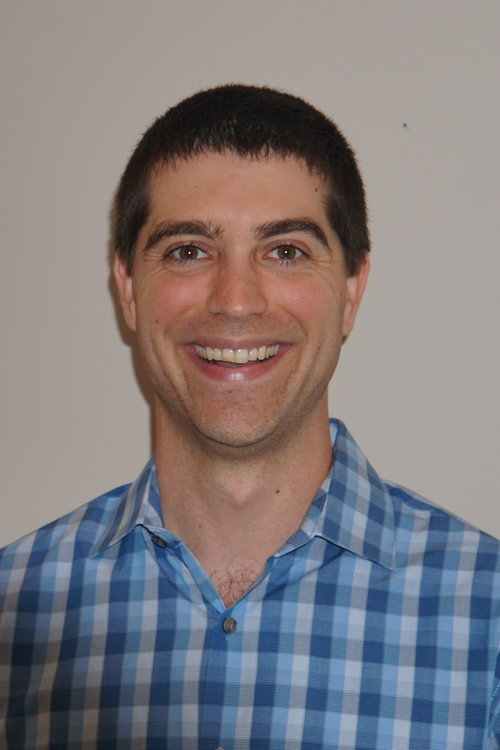
\includegraphics[width=0.9\textwidth]{danneman_headshot.jpeg}
%     \end{center}
%\end{column}
%\end{columns}
%\end{frame}


%\-\hspace{1cm}  indented text


\section{Introduction}

\frame{
\frametitle{Acknowledgements}
Big thanks to:
\begin{itemize}
\item Charlotte Data Science, Machine Learning and AI Meetup
\item Bojana and Maithili
\item Data Machines (www.datamachines.io)
\item DARPA
\end{itemize}

\bigskip
\bigskip
\bigskip
\bigskip
\bigskip

\textcolor{gray}{DISTRIBUTION STATEMENT A: Approved for public release.}
% hyperlink
% \href{url}[link_text}

}


\frame{
\frametitle{Outline}
\begin{enumerate} 
\item Just enough theory/background
\item Feed forward neural networks
\item Convolutional neural networks
\item Use case: Mask fusion for image manipulation localization
\end{enumerate}
}

\frame{
\frametitle{About This Talk}
Goals:
\begin{itemize} 
\item Give you nodding familiarity and ample pointers
\item Leave you a starter code-base
\end{itemize}
\bigskip
This talk lightly assumes:
\begin{itemize}
\item some familiarity with Python
\item knowledge of general data science concepts
\end{itemize}
}


\frame{
\frametitle{Supervised Models Are Function Approximators}


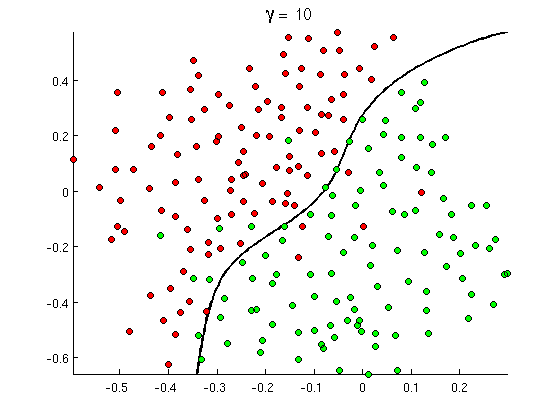
\includegraphics[width=8cm]{func_appox}


}

% What is the plan for teaching FFNNs?

% First, show an image of a simple one, and deal with some nomenclature
% Then, dive into a single neuron
% Then, reminder of the point: function approximaiton
% Learn the weights and biases via SGD and loss

% Show a simple, worked example

% Zoom back out to talk about ALL the hyperparameters, and use that cool dashboard
%% Structural:
% Number of hidden layers
% Number of nodes per layer
%% Smaller:
% Regularization
% Dropout
% Early termination

% Mention: in large models (millions of params) hyperparameter tuning can be EXPENSIVE
\section{Feed Forward Neural Networks}


\frame{
\frametitle{The Feed Forward Neural Network}
\makebox[\textwidth]{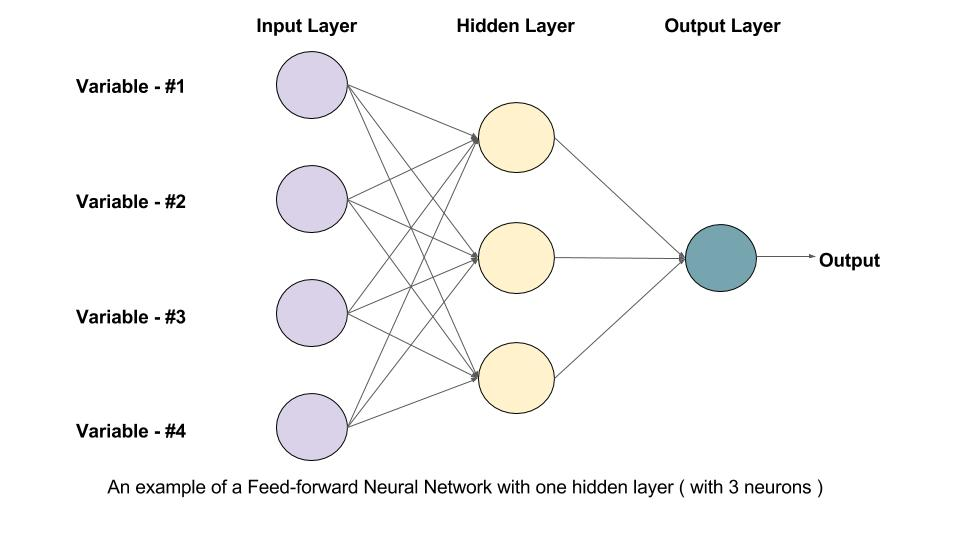
\includegraphics[width=\paperwidth]{ffnn_image.jpg}}
%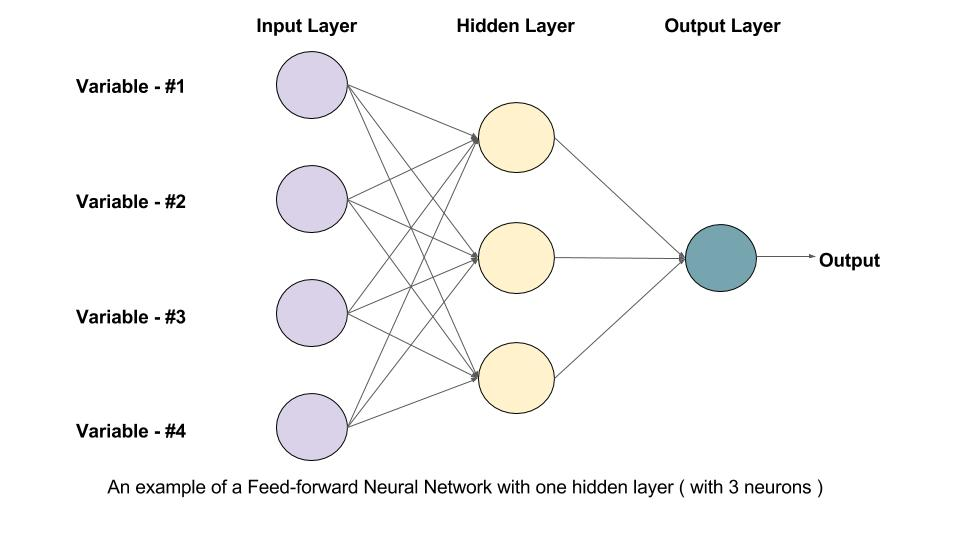
\includegraphics[width=12cm]{ffnn_image.jpg}

% This is a Directed, Acyclic Graph (DAG) that represents a model STRUCTURE

% Input layer: takes in a vector, X, of size four
% These purple circles are just input data
% Hidden layer: has learnable parameters that do transformations
% These beige circles are "neurons", more on that in a minute.
% Output layer: hopefully matches Y closely
% This blue circle is also a neuron.

}


\frame{
\frametitle{Neurons}
Neurons take in the outputs of upstream neurons (or raw data).\\
\smallskip
They multiply that by a matrix of \textbf{weights}.\\
\smallskip
Add a \textbf{bias} term.\\
\smallskip
And pass that entire sum through an \textbf{activation function}.\\
\bigskip
For inputs X, weight matrix W, bias b, and activation function f:\\
\bigskip
Neuron output $ = f(WX + b)$

}

\frame{
\frametitle{Activation Functions}
\makebox[\textwidth]{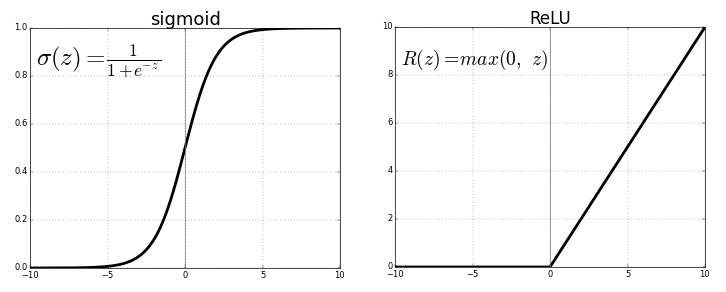
\includegraphics[width=\paperwidth]{sigmoid_relu}}
%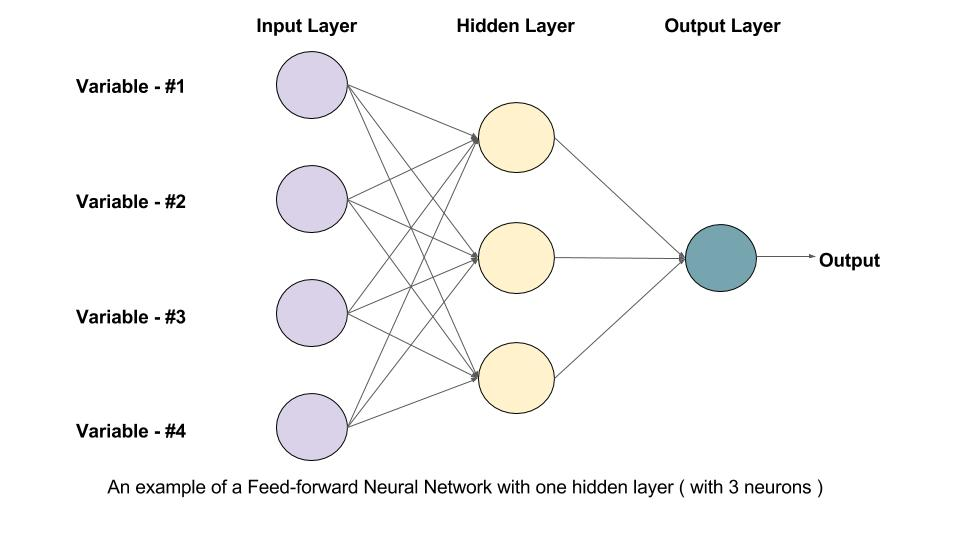
\includegraphics[width=12cm]{ffnn_image.jpg}

}

\frame{
\frametitle{Understanding a Neuron}
\makebox[\textwidth]{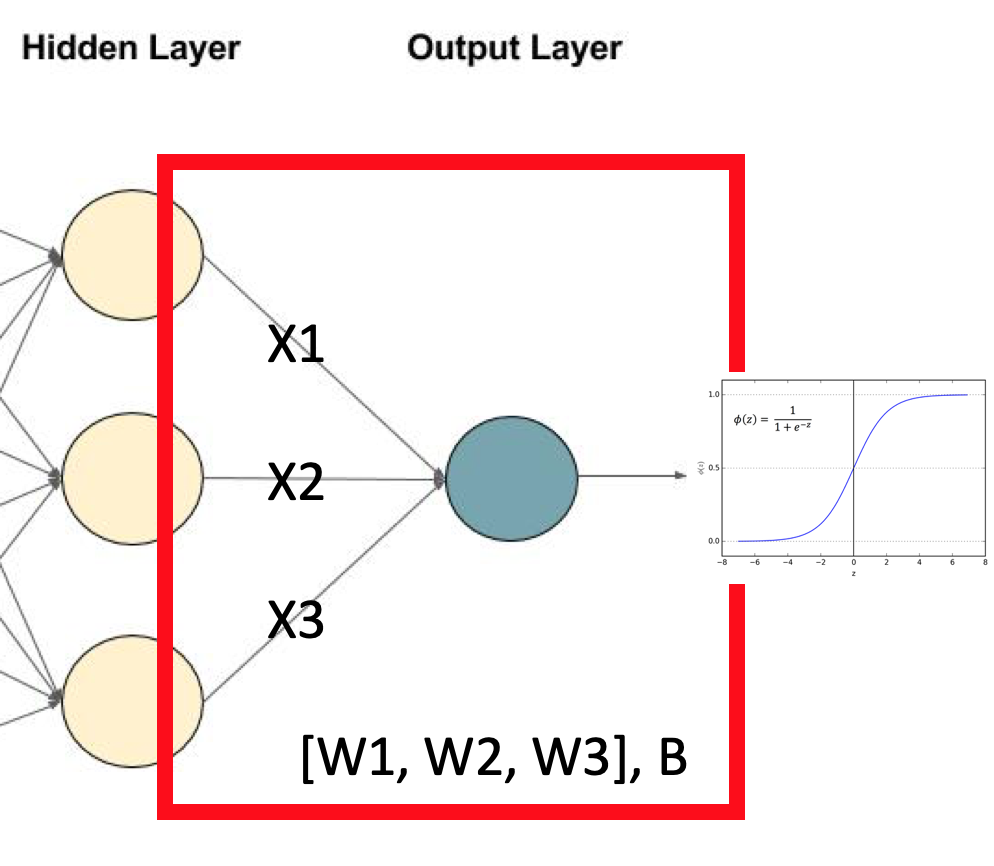
\includegraphics[width=9cm]{neur}}
%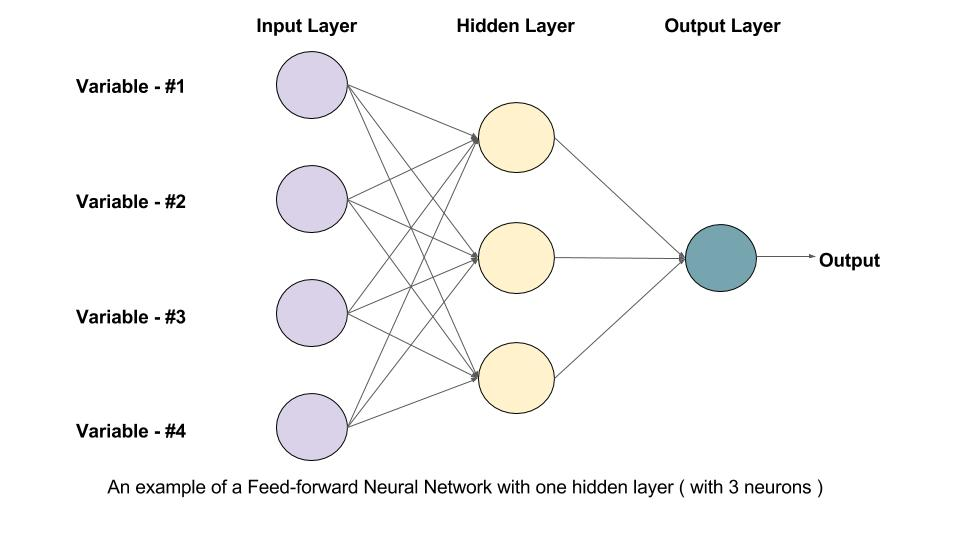
\includegraphics[width=12cm]{ffnn_image.jpg}

}


\frame{
\frametitle{Learning/Estimation/Function Approximation}
Remember: The point is (flexible) function approximation.\\
\bigskip
In this case, approximation is optimization with respect to a \textbf{loss function}.

\bigskip
We \textbf{learn} the weights and biases via stochastic gradient descent.\\

%\bigskip
%
%All models are wrong...some models are useful.
%\bigksip
%A good model approximates x to y in your training data, conditional on the model (in this case I mean the structure...neurons, layers, activations, other params not yet mentioned) you've specified.
% Say something about what that is.
% Reminder: Keras does all this for you...but you have to pick some parameters of the learning itself
% More on that later.

}


\frame{
\frametitle{What is Keras?}
Light wrapper over TensorFlow.\\
\medskip
https://keras.io\\
\medskip
APIs allow simplicity and still power.\\
\medskip
Great for \textbf{using} neural networks, even very complex ones.\\
\medskip
Poor for research  \textbf{on} neural networks.
}


\begin{frame}[fragile]
\frametitle{Setup}
pip install keras\\
\medskip
 -- it brings along TensorFlow, numpy, etc\\
\medskip
(that was easy)\\
\medskip
Setup for GPU usage
\end{frame}

%\begin{frame}[fragile]
%\frametitle{...}
%\end{frame}


\frame{
\frametitle{Code Example: Iris Classification}

\begin{center}

\makebox[\textwidth]{

\begin{tabular}{ ccccc } 
 \hline
 Sepal Length & Sepal Width & Petal Length & Petal Width & Species \\ 
 7.0 & 3.2 & 4.7 & 1.4 & versicolor \\
 ...&...&...&...&...\\
 ...&...&...&...&...\\
 5.9 & 3.0 & 5.1 & 1.8 & virginica \\
 \hline
\end{tabular}
} % close box

\end{center}
}

\begin{frame}[fragile]
\frametitle{A Simple Model}
\begin{verbatim}
model = Sequential()

model.add(Dense(3, input_dim=4))
model.add(Dense(5))
model.add(Dense(3, activation='sigmoid'))

optimizer_details = SGD(lr=0.01, decay=1e-6)
model.compile(loss='binary_crossentropy',
              optimizer=optimizer_details)

model.fit(X_train, Y_train, epochs=20)
\end{verbatim}
\end{frame}




\frame{
\frametitle{Hyperparameters and Overfitting}

Hyperparameters:
\begin{itemize}
 \item Number of layers
 \item Number of neurons in each layer
\end{itemize}
\bigskip

Strategies to avoid overfitting:
\begin{itemize}
\item Premature halting
\item Dropout
\item Regularization
\end{itemize}

\bigskip
Visit \textcolor{blue}{http://playground.tensorflow.org} to see how hyperparameters affect outcomes in real models of toy data.
}



\frame{
\frametitle{Pragmatics}
\begin{itemize}
\item Start with an overly expressive model
\item Track measure(s) of interest on test data; terminate upon plateau
\item Match the problem type, output layer, and loss function
\end{itemize}
\begin{center}

\makebox[\textwidth]{

\begin{tabular}{ ccc } 
 \hline\hline
 Problem Type & Output Layer & Loss Function  \\ 
 \hline
 Regression & 1-unit Linear & Mean Squared Error \\
 Binary Classification & 1-unit Sigmoid  (softmax) & Binary Crossentropy \\
 k-Class Classification & k-unit Sigmoid (softmax) & Categorical Crossentropy \\

 \hline
\end{tabular}
} % close box

\end{center}

}



\frame{
\frametitle{Applicability}
Q: When might you use a feed-forward neural network for regression or classification?\\
\bigskip
\bigskip
A: Probably never.
}


\section{Image Classification with CNNs}


\frame{
\frametitle{Image Classification with Neural Networks}

Where \textbf{do} people get value out of neural nets? \\

\bigskip

\bigskip

\pause

Images are arrays: Height by Width by 3 (RGB) \\
\medskip
Why not ``unwrap'' them then use a set of fully connected layers?\\

\bigskip
\begin{itemize}
\item Tons of parameters
\item Pixel location is relative
\end{itemize}
}

\frame{
\frametitle{Convolutional Neural Network (CNN)}

Conv Nets solve those problems by:\\

\smallskip

\begin{itemize}
\item Parameter sharing
\item Looking at an image hierarchically
\end{itemize}

\bigskip
Idea:

\begin{itemize}
\item Find a set of micro-pictures that roughly capture the content across patches of all images (convolution)
\item Then, let a single pixel represent its neighborhood, dropping the rest of the information (pooling)
\item Repeat, generating a hierarchical view
\end{itemize}


}

\frame{
\frametitle{Convolutional Filters}
``Find a set of micro-pictures that roughly capture content in every patch of all images''\\
\bigskip
\bigskip

\makebox[\textwidth]{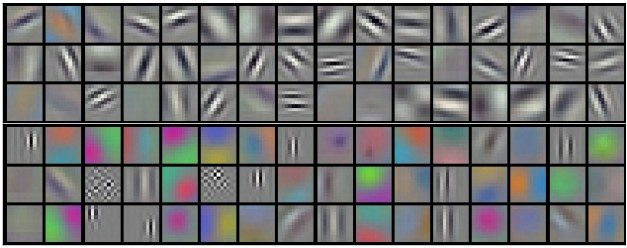
\includegraphics[width=8cm]{filters}}

}


\frame{
\frametitle{Pooling Operation}
``Let a single pixel represent how much each filter matches the surrounding patch'' \\
\bigskip
\bigskip

\makebox[\textwidth]{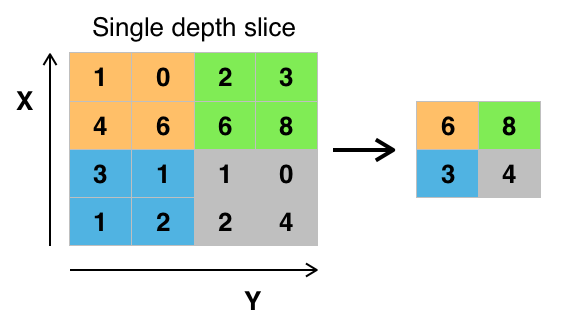
\includegraphics[width=8cm]{pooling}}

}

\frame{
\frametitle{Repeat for Hierarchical Image Description}

\makebox[\textwidth]{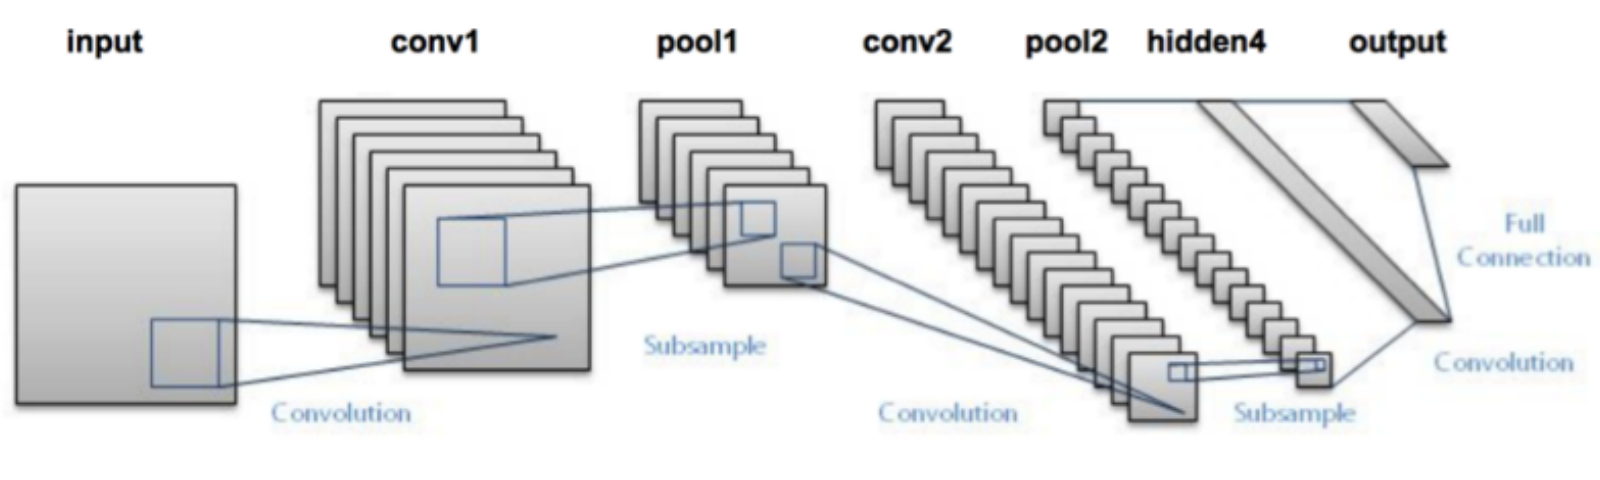
\includegraphics[width=12cm]{arch}}

\medskip

To learn:
\begin{itemize}
\item filters (which are just weights and biases with structure)
\item weights and biases for hidden/output layers
\end{itemize}

}


\begin{frame}[fragile]
\frametitle{A Tiny Example: Model Setup}
\begin{verbatim}
from keras import Sequential
from keras.layers import Conv2D, MaxPooling2D, Dense
from keras.layers import Flatten
from keras.optimizers import SGD

model = Sequential()
model.add(Conv2D(32, kernel_size=(5, 5), 
	input_shape=input_shape))
model.add(MaxPooling2D(pool_size=(2, 2)))
model.add(Flatten())
model.add(Dense(50, activation='relu'))
model.add(Dense(num_classes, activation='softmax'))
\end{verbatim}
\end{frame}

\begin{frame}[fragile]
\frametitle{A Tiny Example: Model Fitting}
\begin{verbatim}
model.compile(loss=categorical_crossentropy,
              optimizer=SGD(lr=0.01),
              metrics=['accuracy'])

model.fit(x_train, y_train,
          batch_size=batch_size,
          epochs=epochs,
          verbose=1)
\end{verbatim}
\end{frame}



\frame{
\frametitle{Some Pragmatics}

\begin{itemize}
\item Are your images special? 
\begin{itemize}
\item This is unlikely; consider fine-tuning an existing model.
\end{itemize}
\item Are your images all the same size?
\begin{itemize}
\item Either resize or consider pyramidal layers.
\end{itemize}
\item Are your images large? Or many of them?
\begin{itemize}
\item You likely need a GPU
\end{itemize}
\end{itemize}

}


\frame{
\frametitle{A Challenging Use Case}
Program Challenge: Write software that identifies altered images \\
\medskip
Researchers write analytics that output scores and masks \\
\medskip
My team tries to \textbf{fuse} the masks into a single, optimal mask.
}



%\begin{frame}
%\frametitle{Mask Fusion - Details}
%\begin{columns}
%\begin{column}{0.4\textwidth}
%Challenges:
%\begin{itemize}
%\item Missing data
%\item Chunky masks
%\item Heterogeneous image sizes
%\end{itemize}
%\end{column}
%\begin{column}{0.6\textwidth}
%    \begin{center}
%     \includegraphics[width=.99\textwidth]{cat_mask}
%     \includegraphics[width=.4\textwidth]{chunky}
%     \end{center}
%
%\end{column}
%\end{columns}
%\end{frame}

\begin{frame}
\frametitle{Example Data}
\begin{columns}
\begin{column}{0.5\textwidth}
    \begin{center}
     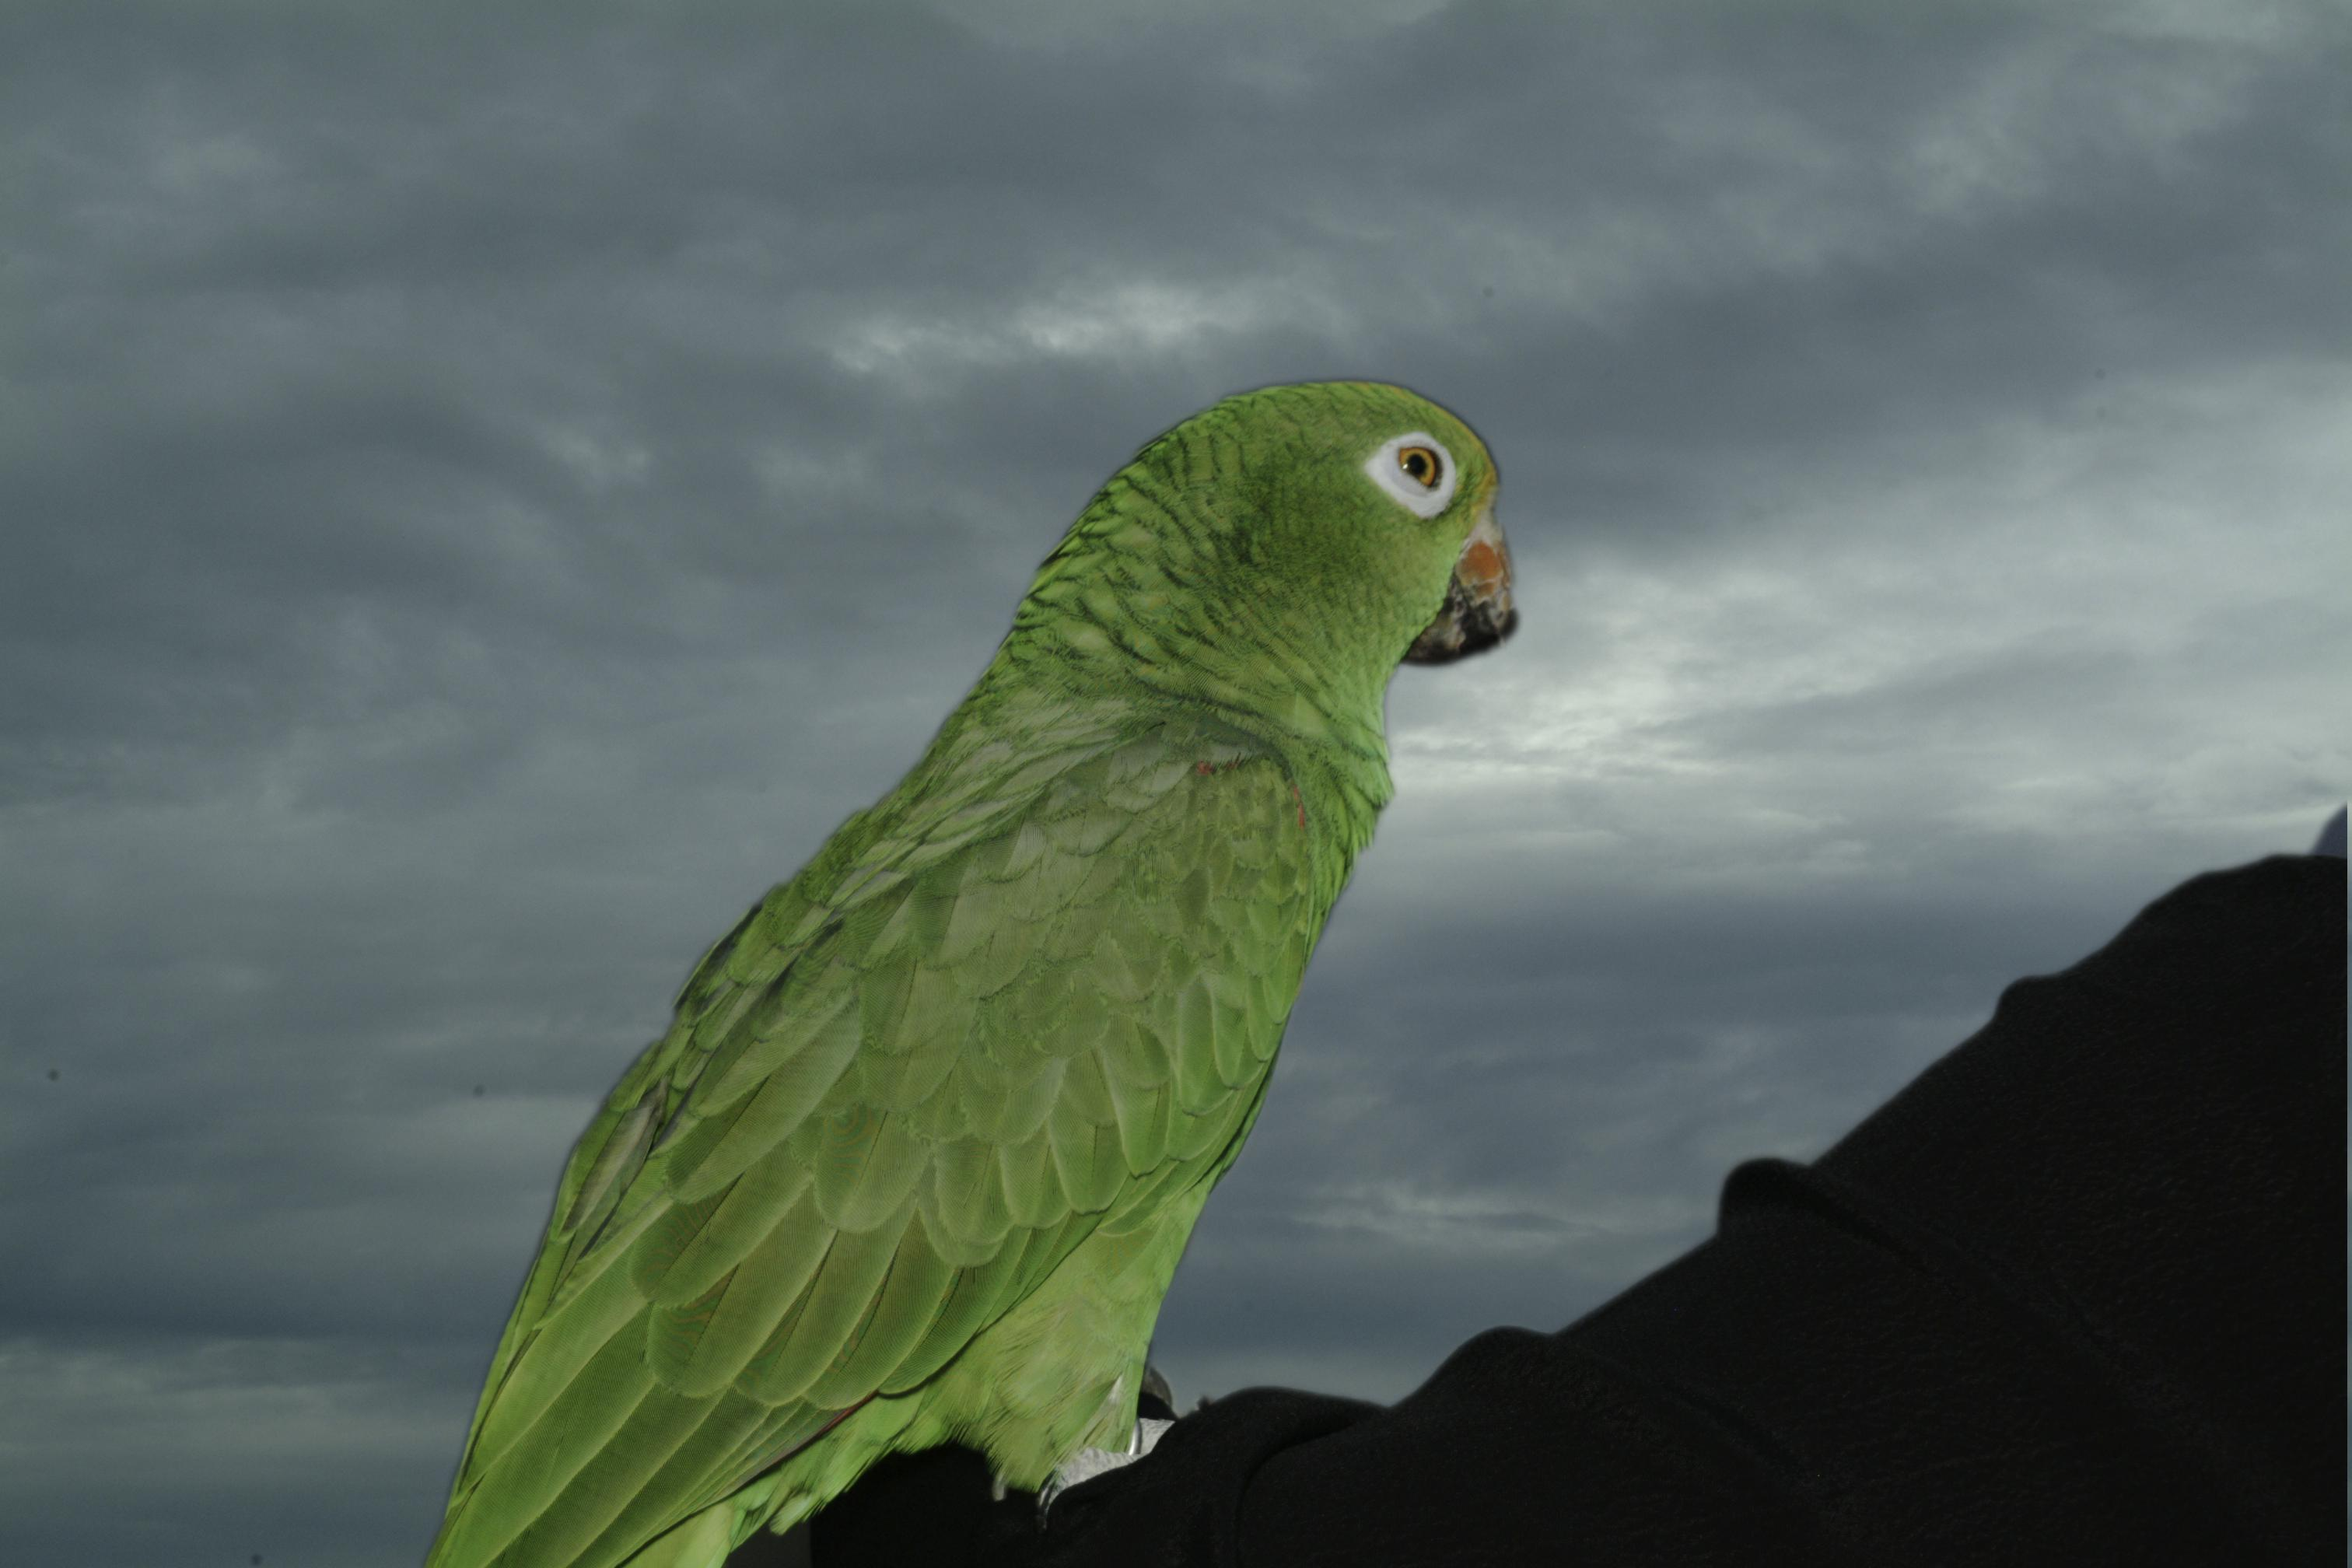
\includegraphics[width=.9\textwidth]{mask_real}
     \end{center}
\end{column}
\begin{column}{0.5\textwidth}
    \begin{center}
     
\includegraphics[width=.9\textwidth]{mask_1}
     \end{center}

\end{column}
\end{columns}
\end{frame}

\begin{frame}
\frametitle{Example Data}
\begin{columns}
\begin{column}{0.5\textwidth}
    \begin{center}
     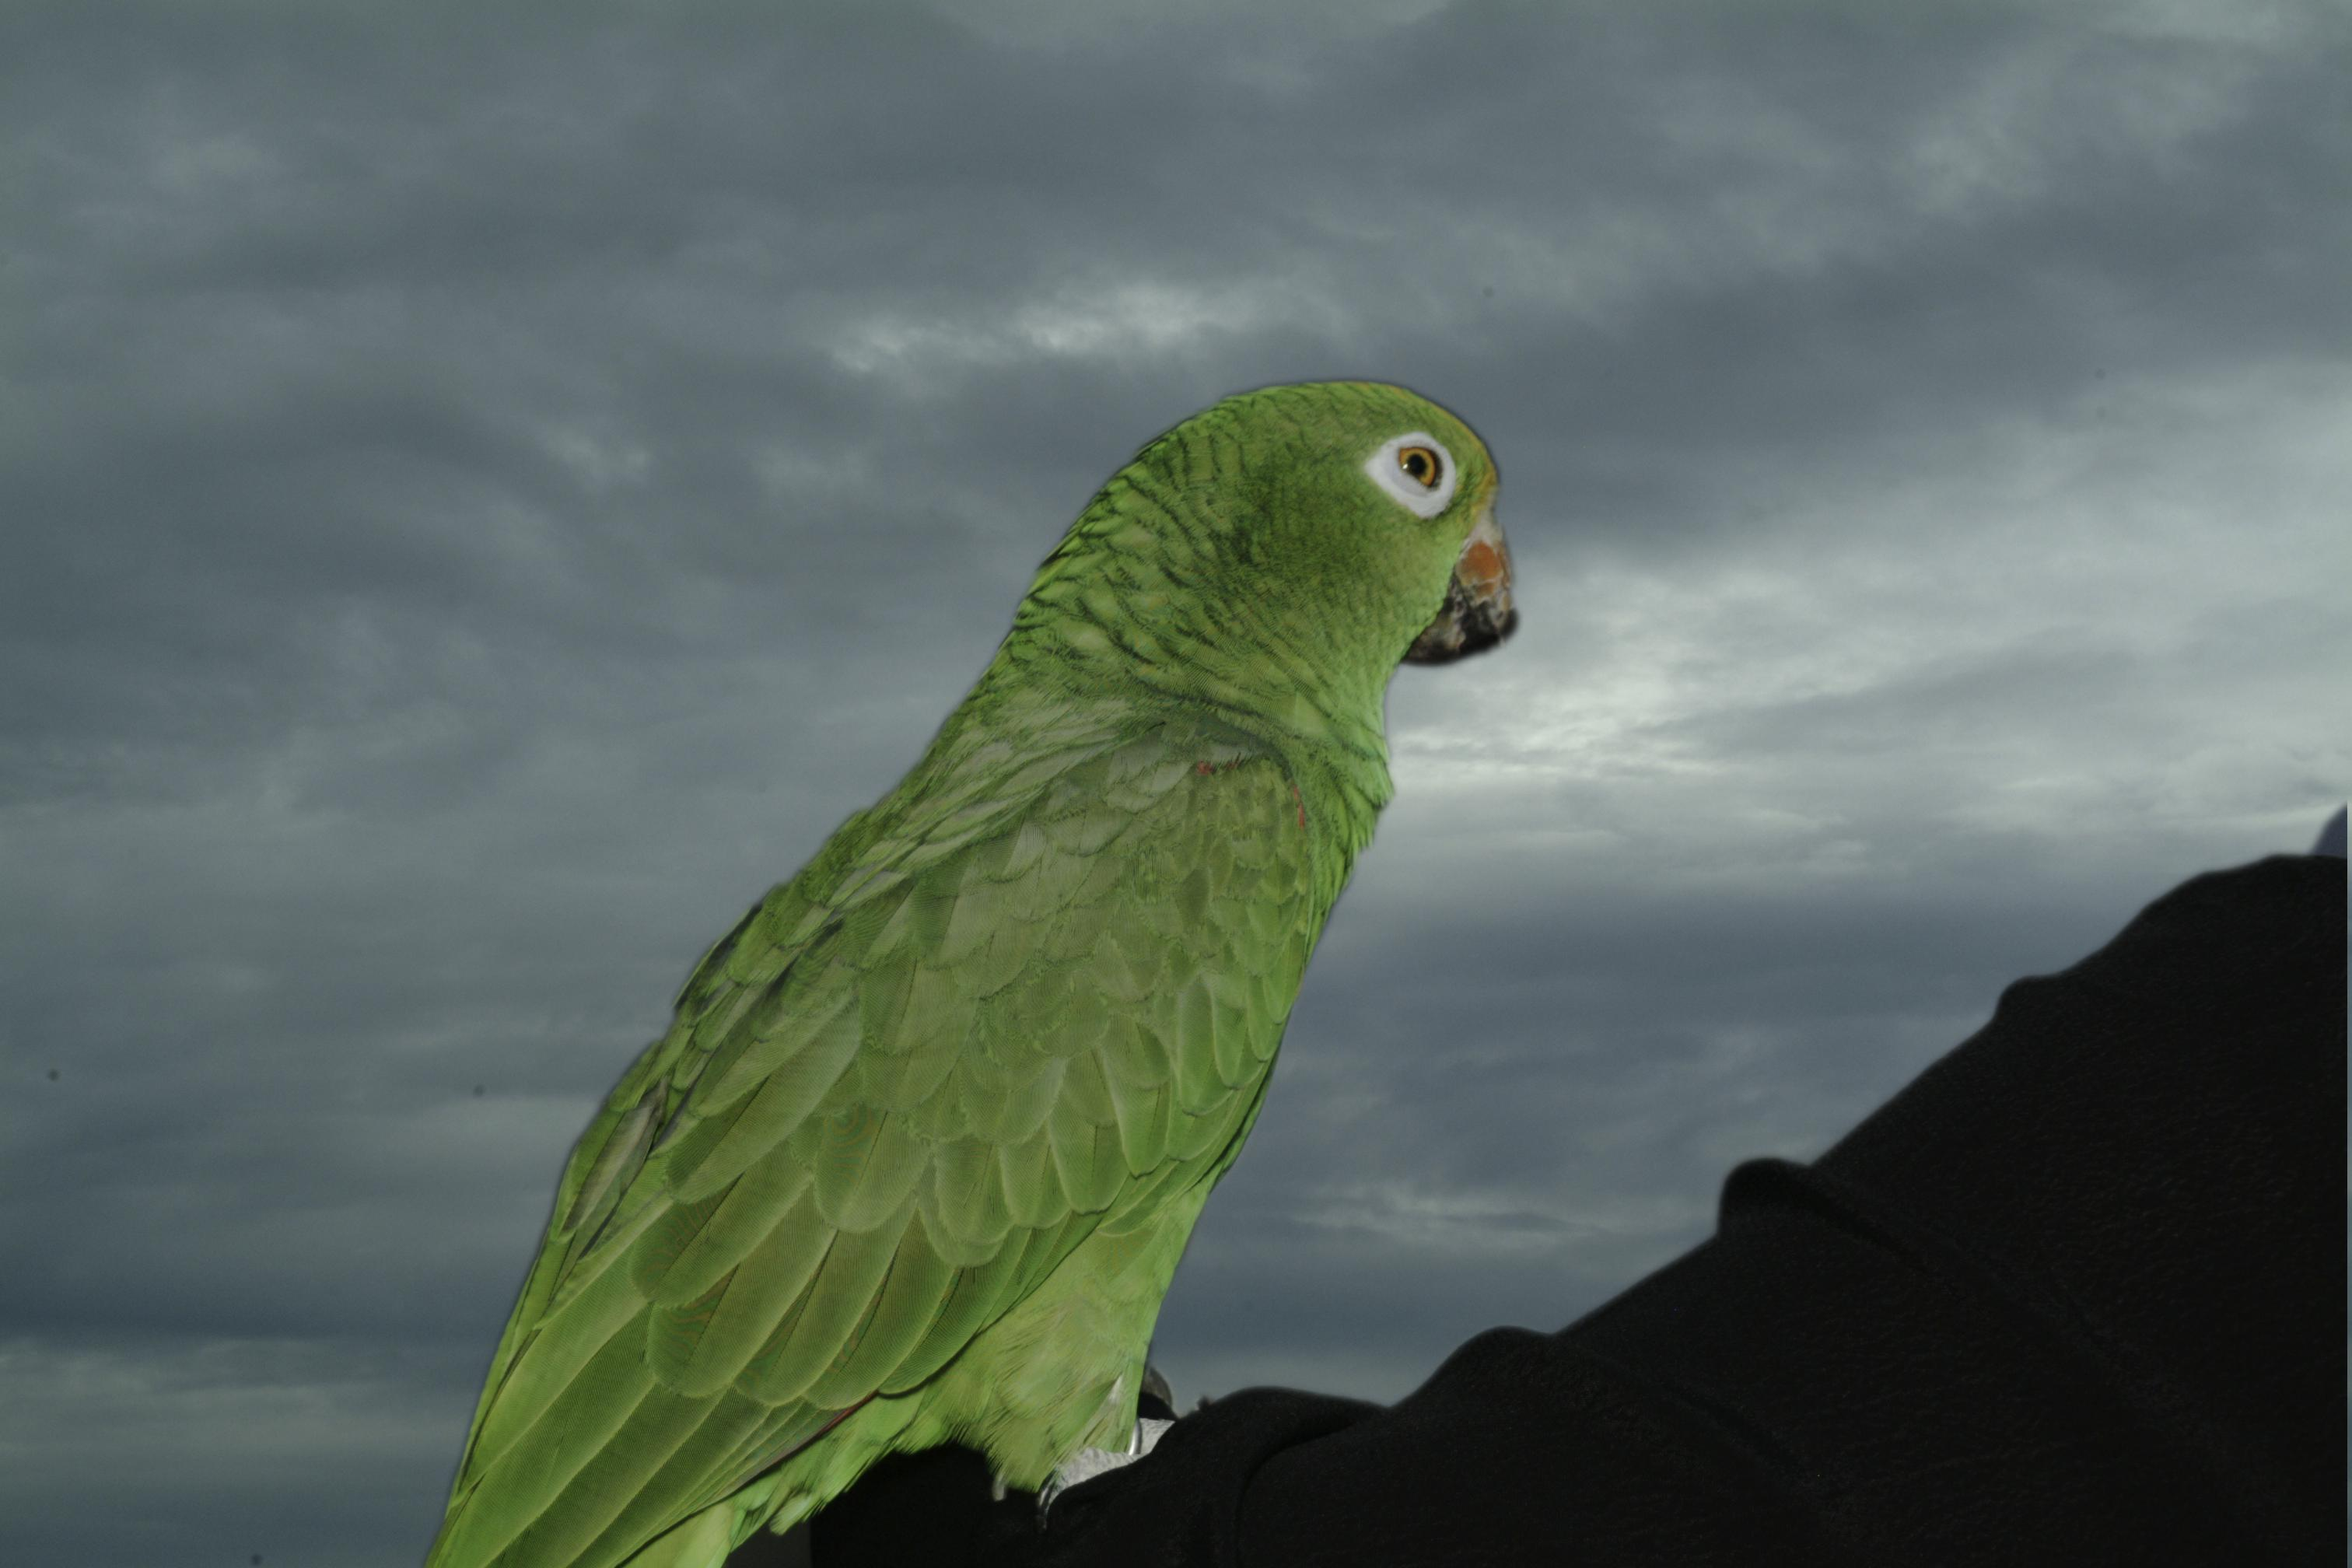
\includegraphics[width=.9\textwidth]{mask_real}
     \end{center}
\end{column}
\begin{column}{0.5\textwidth}
    \begin{center}
     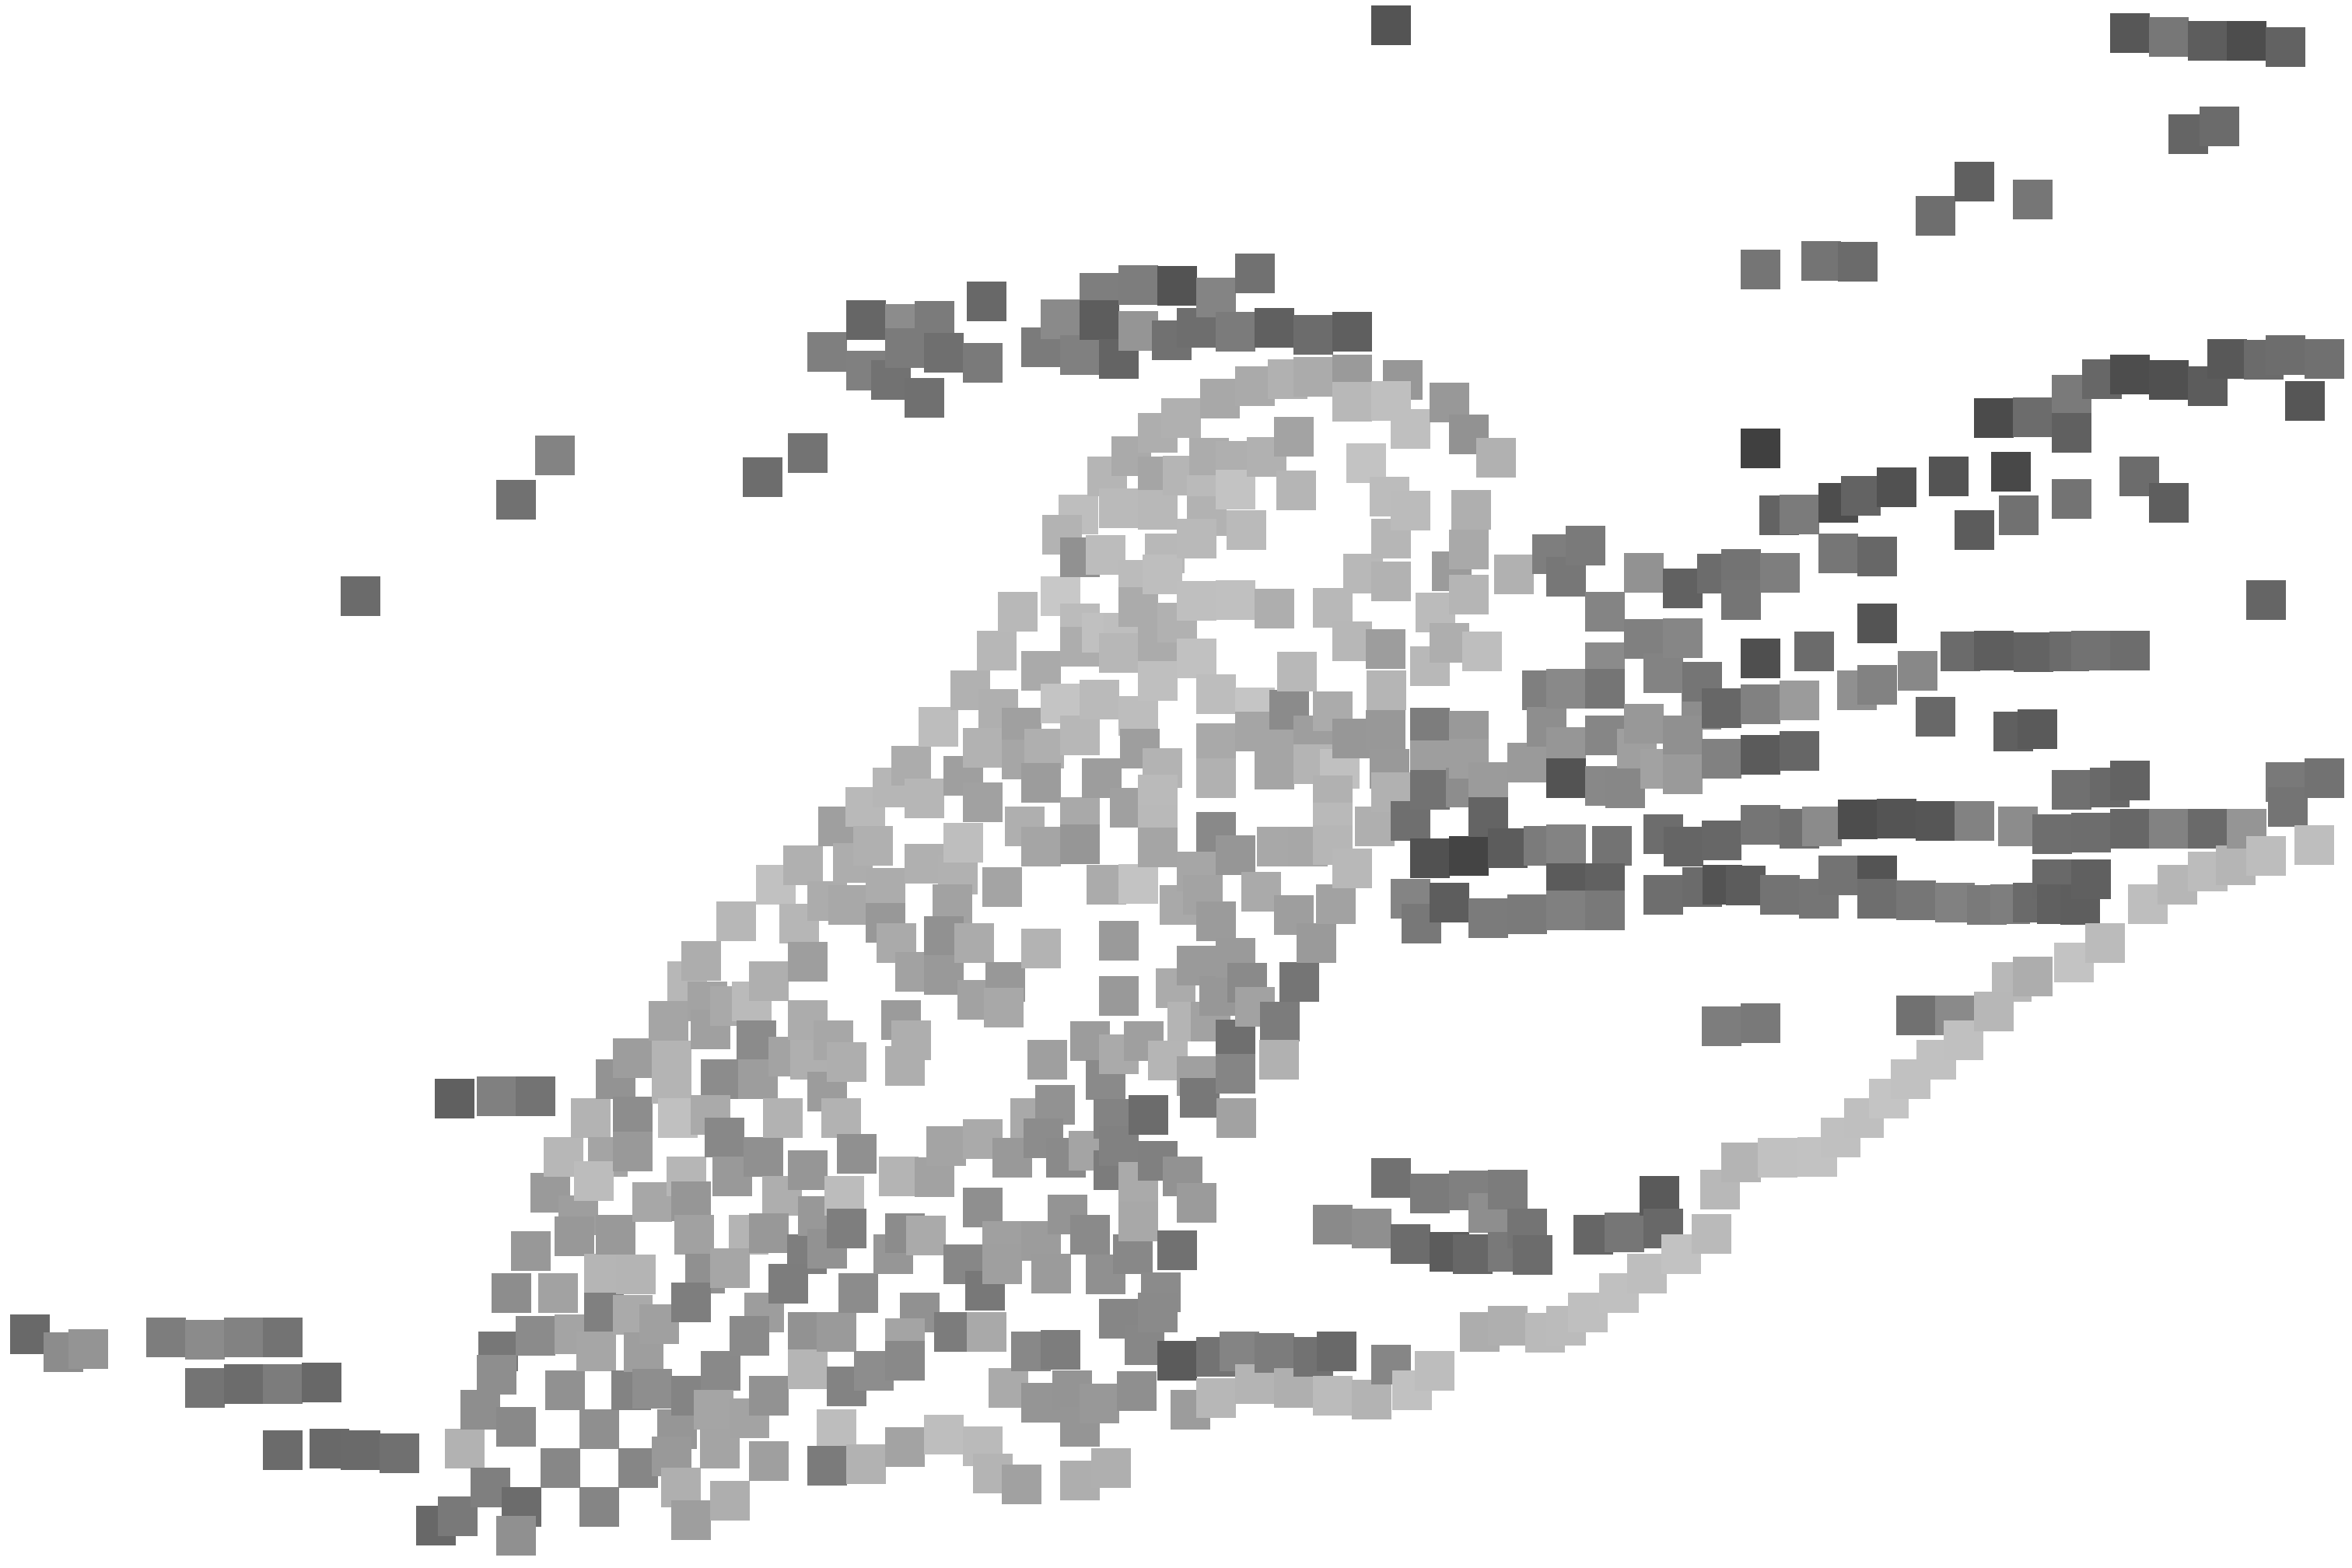
\includegraphics[width=.9\textwidth]{mask_2}
     \end{center}

\end{column}
\end{columns}
\end{frame}

\begin{frame}
\frametitle{Example Data}
\begin{columns}
\begin{column}{0.5\textwidth}
    \begin{center}
     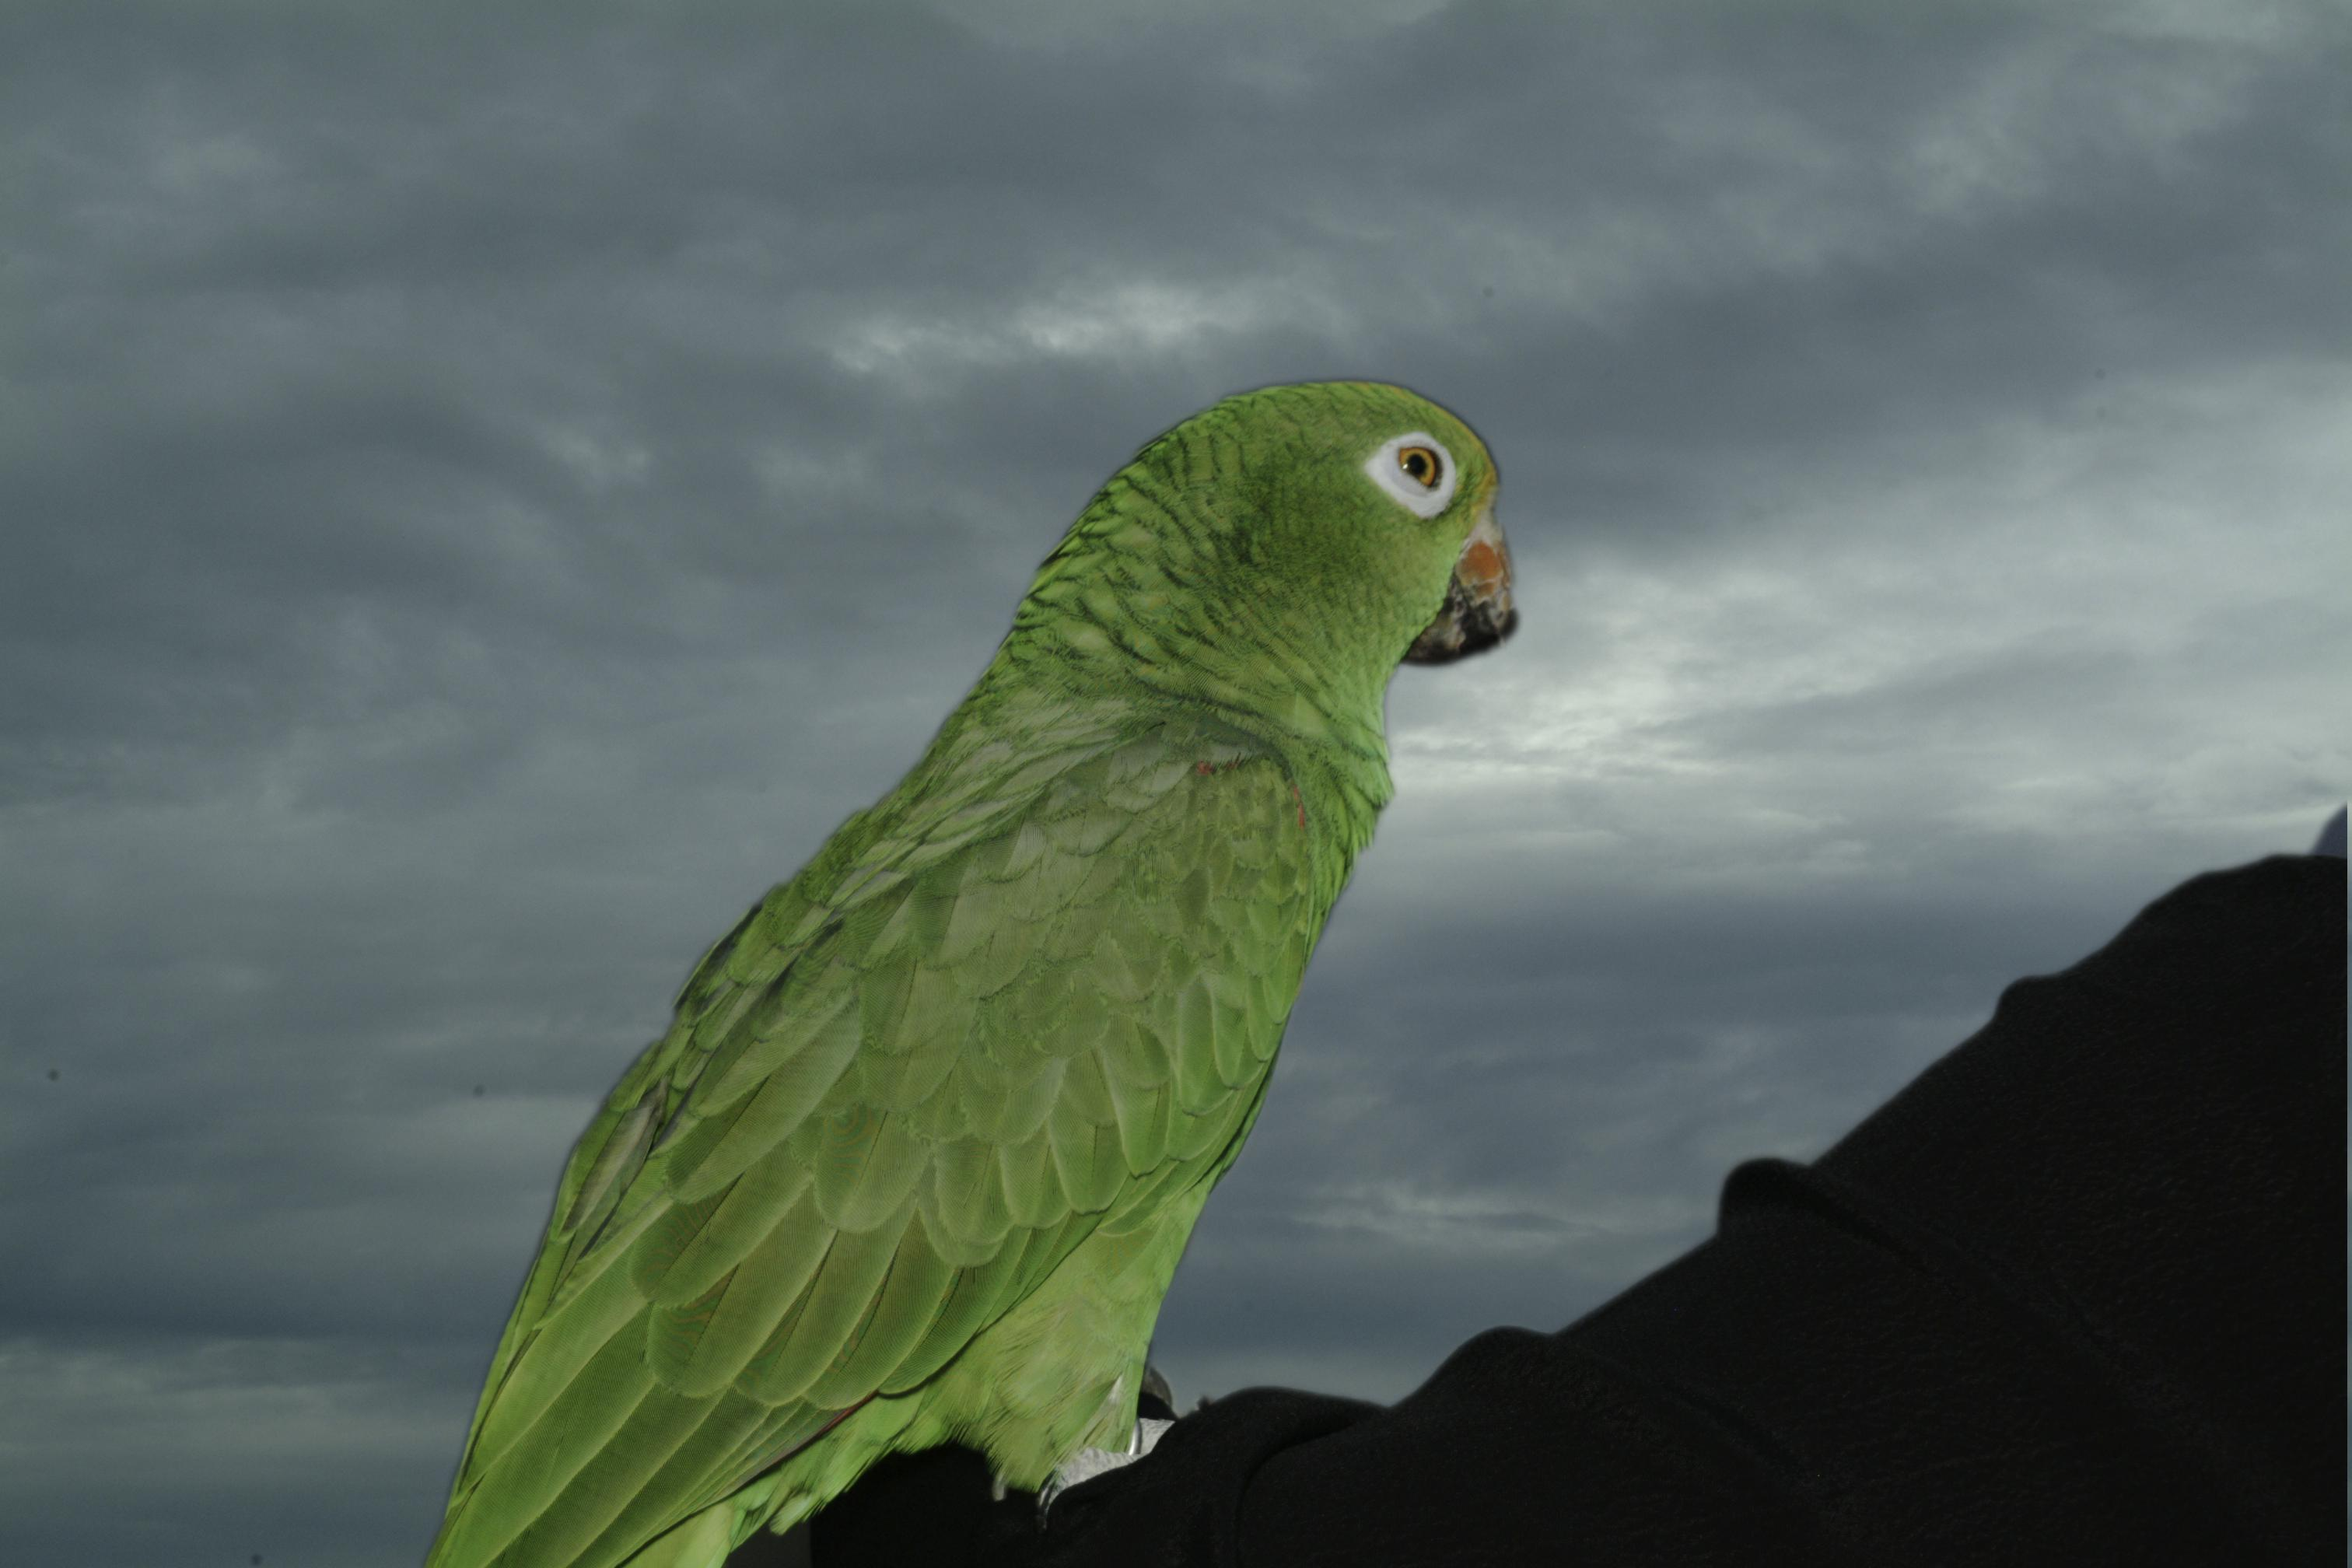
\includegraphics[width=.9\textwidth]{mask_real}
     \end{center}
\end{column}
\begin{column}{0.5\textwidth}
    \begin{center}
     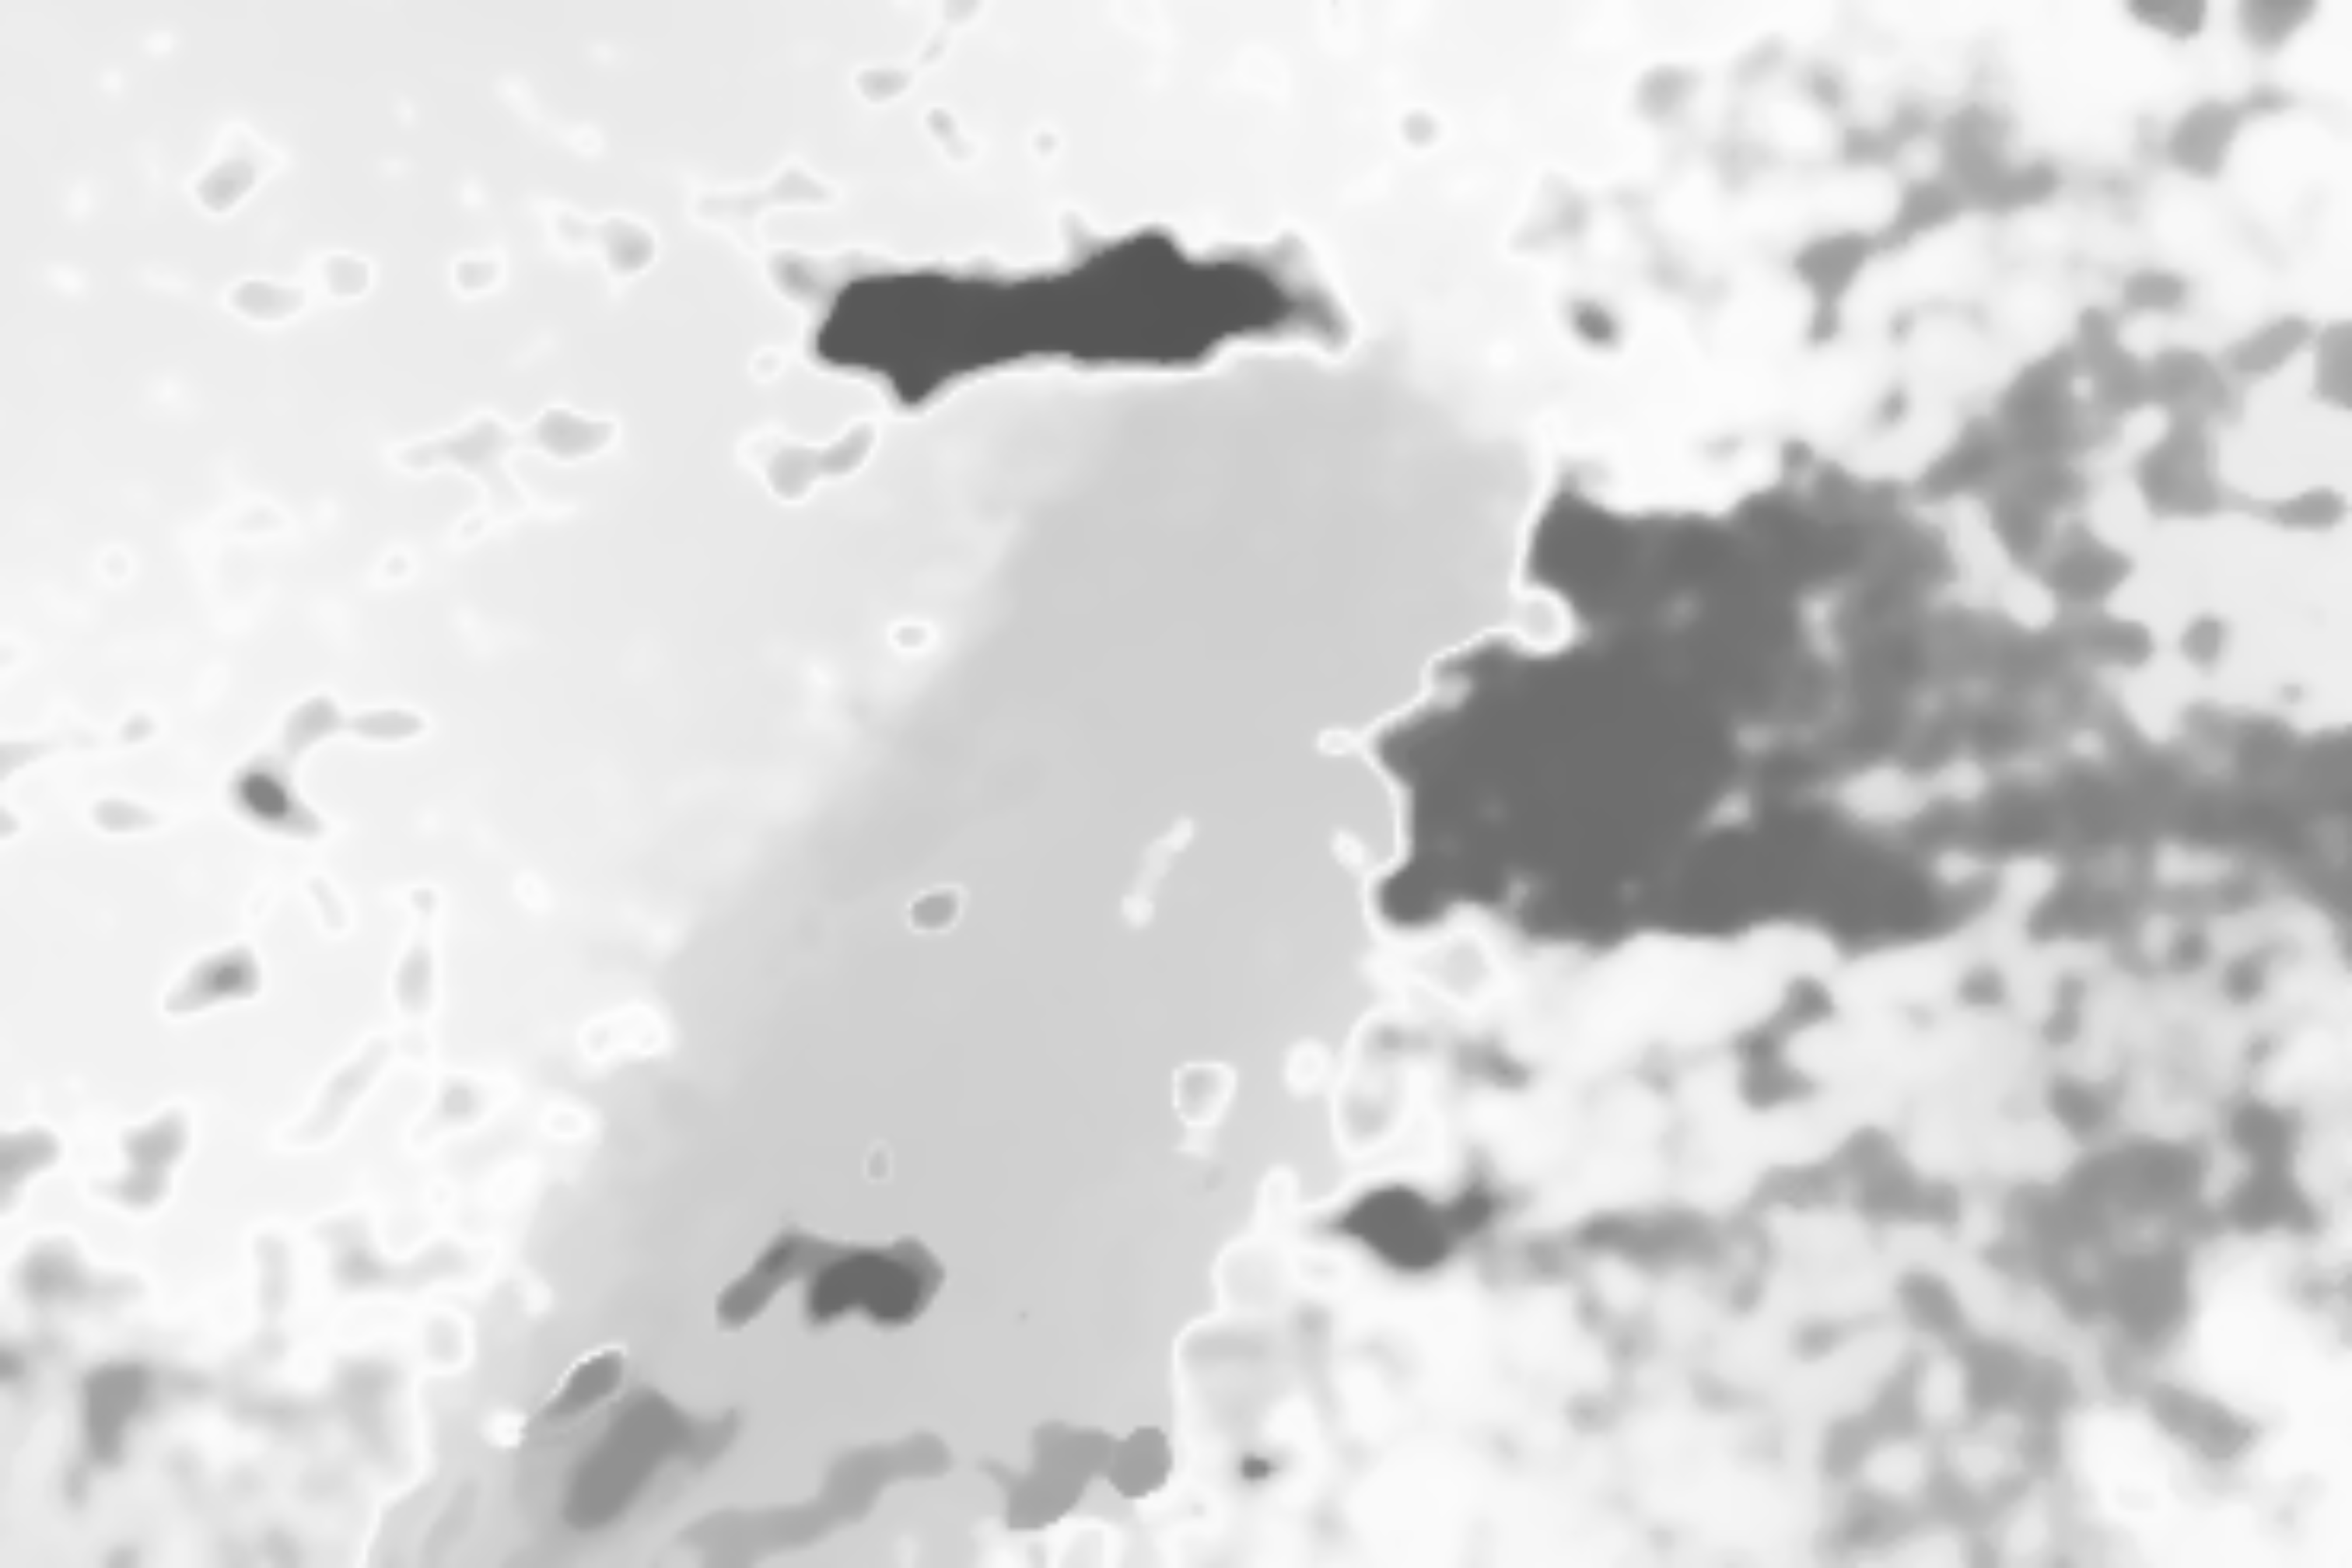
\includegraphics[width=.9\textwidth]{mask_3}
     \end{center}

\end{column}
\end{columns}
\end{frame}


\frame{
\frametitle{Mask Fusion: Some Intuition}
\begin{itemize}
\item Spatial smoothing
\item Handle missing data
\item Lightly parameterized -- modest data
\item Output is same shape as input image
\end{itemize}
}


\frame{
\frametitle{Approach}
\begin{itemize}
\item Large filters for spatial smoothing
\item Not too deep a model (fewer paramters)
\item Sized all images to 128x128, resize output back to original shape
\item Missing data placeholder to -1
\end{itemize}

\bigskip
Eventually: Added information from an image segmentation model.
}


\begin{frame}[fragile]
\frametitle{Example Autoencoding Setup}
\begin{verbatim}
mod = Sequential()
# Encoder Layers
mod.add(Conv2D(18, (4,4), input_shape=(256, 256, 27)))
mod.add(BatchNormalization())
mod.add(MaxPooling2D((4,4), padding='same'))
# Decoder Layers
mod.add(UpSampling2D((4,4)))
mod.add(Conv2D(1, (4,4), activation='sigmoid'))
\end{verbatim}
\end{frame}


\frame{
\frametitle{Results}
Short Version: Better than the best single analytic by a large margin.
}


\frame{
\frametitle{Resources}
\begin{itemize}
\item Keras:  https://keras.io
\item Keras tutorial:  https://elitedatascience.com/keras-tutorial-deep-learning-in-python
\item Intro to CNNs:  https://towardsdatascience.com/simple-introduction-to-convolutional-neural-networks-cdf8d3077bac
\item Mathy intro to CNNs: https://arxiv.org/pdf/1511.08458.pdf
\item Advanced CNN architectures: https://slazebni.cs.illinois.edu/spring17/lec04\_advanced\_cnn.pdf
\item Hyperparameter tuning:  http://playground.tensorflow.org
\end{itemize}
}

%\frame{
%\frametitle{}
%
%}


%\frame{
%\frametitle{}
%
%}



%
%
%\frame{
%\frametitle{Language Modeling as Sequence Modeling}
%Most language is treated as sequences of tokens.
%The tokens are typically lowercase, lemmatized words.
%Though some models include much more (e.g. Bert).
%
%
%}
%
%\frame{
%\frametitle{What's a Sequence Model?}
%Try to predict the next token from the previous x tokens (i.e. Markov Model).
%Try to come up with an embedding that represents a sequence or its type (i.e. hidden Markov Model).
%}
%
%\frame{
%\frametitle{Long Short-term Memory Models (LSTM)}
%how these work.
%
%some details...er...
%
%}
%
%\frame{
%\frametitle{A Fun Example:}
%Who said it: XX or YY.
%}

%\frame{
%\frametitle{}
%
%}

%\frame{
%\frametitle{}
%
%}

%\frame{
%\frametitle{}
%
%}

%\frame{
%\frametitle{}
%
%}






%
%\frame{
%\frametitle{Defensive Analytics I: Rules}
%Idea: Encode knowledge about known TTPs as rules.\\
%\bigskip
%\begin{itemize}
%\item e.g. Snort \\
%\item If (ip AND port OR domain) then (block/report/etc) \\
%\pause
%\item Pros: understandable, targeted, fast (to implement and execute)\\
%\item Cons: simplistic; known-knowns; short shelf-life
%\end{itemize}
%}
%
%
%\frame{
%\frametitle{Defensive Analytics II: Statistical Pattern Matching}
%Idea: Train a model to differentiate malicious cases from safe ones.\\
%\bigskip
%\begin{itemize}
%\item e.g. FireEye \\
%\item Statistical model separating, e.g., malware-containing .doc(x) from safe examples
%\pause
%\item Pros: targeted, accurate \\
%\item Cons: need training data; uninterpretable models; short shelf-life; need many models to achieve broad coverage
%\end{itemize}
%}
%
%\frame{
%\frametitle{Defensive Analytics III: Statistical Anomaly Detection}
%Idea: Use a statistical model to highlight anomalous activity.\\
%\bigskip
%\begin{itemize}
%\item e.g. IronNet \\
%\item Either model normalcy and alert on deviations, or directly estimate ``anomalousness''
%\pause
%\item Pros: dynamic models; per-environment customization; detect unknowns  \\
%\item Cons: noisy; definition of ``anomaly'' implies algo implies variance in results; uninterpretable
%\end{itemize}
%}
%
%
%\frame{
%\frametitle{Best of All Worlds?}
%RuleBreaker attempts to get some of the power of each approach, while avoiding each one's pitfalls.\\
%\bigskip
%
%Idea: generate simplified models of normalcy in the form of probabilistic rules.
%
%\bigskip
%\begin{itemize}
%\item Dynamism and `unknown unknowns' of anomaly detection \\
%\item Interpretability of rules \\
%\item Accuracy of statistical pattern matching
%\end{itemize}
%
%}
%
%
%\frame{
%\frametitle{Motivation}
%Network data, through RFCs and convergent usage patterns, often includes strong interdependencies between fields.
%\bigskip
%\begin{itemize} 
%\item File extensions imply mime\_type.\\
%\item Port 53 traffic + AAAA record implies range of return bytes.\\
%\item Port number correlates strongly with protocol.
%\end{itemize}
%\bigskip
%Idea: Automatically identify strong, categorical correlations to \textcolor{red}{learn about a network}. \\
%\bigskip
%Then, find observations that break them, to \textcolor{red}{identify anomalies}.
%}
%
%\frame{
%\frametitle{Further Motivation}
%
% \begin{overlayarea}{\textwidth}{0.23\textheight}
% \visible<1>{
%\includegraphics[width=1.9cm]{thinking_face}
%\end{overlayarea}
%}
%\visible<1->{
%Can't we just use SQL to find these?
%}
%\visible<2->{
%\begin{itemize}
%\item Yes, \emph{if you already know} what mis-matches you're looking for
%\item Yes, \emph{if there are few mis-matches} you care about
%\end{itemize}
%}
%
%\bigskip
%\visible<3->{
%Hey, isn't this just anomaly detection?
%\begin{itemize}
%\item Yes-ish.
%\item Optimized for categorical data
%\item Performant in the face of irrelevant variables
%\item Focused on `near-misses'
%\end{itemize}
%}
%}
%
%
%\frame{
%\frametitle{The Language of Rules}
%RuleBreaker thinks of categorical correlations as \emph{rules}.\\
%\bigskip
%Example: if DNS, then port 53 with probability 98\%.\\
%\bigskip
%These are \emph{descriptive} rather than \emph{normative}; they are identified from data.\\
%\bigskip
%Rules have three parts: predicate, consequent, and (conditional) likelihood.
%
%}
%
%
%\frame{\frametitle{Inducing Rules from Data}
%Association Rule Mining is the task of identifying antecedent sets that are highly likely to imply consequents.\\ 
%\textcolor{gray}{(ie. find strong correlations in categorical data)}\\
%\bigskip
%Originated with market basked analysis\\
%\textcolor{gray}{(bread + peanut butter $=>$ jelly)}\\
%\textcolor{gray}{see Agrawal, Imielinski, and Swami (1993)}\\
%\bigskip
%Task involves first identifying frequent itemsets \\
%\textcolor{gray}{(bread, peanut butter, jelly)}\\
%\bigskip
%Next, you use those itemsets to identify high-confidence rules\\
%\textcolor{gray}{ \{bread, peanut butter $=>$ jelly 99\% of the time \} }
%}
%
%\frame{\frametitle{Identifying Frequent Itemsets}
%
%A \textcolor{red}{Frequent Itemset} is a set (group of levels of variables) that occurs with higher than S(upport) frequency in a database.\\
%\bigskip
%FP-Growth \textcolor{gray}{(Han et al, 2000)}
%\begin{itemize}
%\item Scan database ONCE to find (sorted list) of frequent items
%\item Grow a tree based on order of frequency
%\item Use the tree structure to rapidly identify frequent itemsets without candidate generation
%%\item Check for confidence of rules made from binary partitions of itemsets
%\end{itemize}
%}
%
%
%\frame{\frametitle{Identifying Rules from Frequent Itemsets}
%A \textcolor{red}{Rule} is a unary split of a set where the likelihood of the consequent given the predicate in the dataset has a minimum \emph{confidence} (percentage).\\
%\bigskip
%
%Itemset: \{A,B,C\}\\
%Unary split: \{A,C\}, \{B\}\\
%Rule: If \{A,C\} then \{B\} with probability 96\%\\
%\bigskip
%
%Rule Induction:
%Generate unary splits of all frequent itemsets, and check the resulting conditional probabilities in the database.
%}
%
%
%\frame{\frametitle{Why Do We Care?}
%
%Learn about \textcolor{red}{patterns} in the network:\\
%
%\begin{itemize}
%\item DNS running over an atypical port
%\item Services associated with username-types
%\item Note proxies
%\end{itemize}
%
%\bigskip
%
%Identify \textcolor{red}{discrepancies}.\\
%E.g. ``IF port=53 THEN protocol=`dns' 99.7\% of cases.''~~~~~(rule)\\
%1.2.3 sent icmp traffic to 4.5.6 over port 53.~~~~~~~~~~~~~~~~(breakage)
%
%}
%
%\frame{\frametitle{How to Generate Security-Relevant Rules}
%
%At a high level, RuleBreaker is anomaly detection. \\
%
%\bigskip
%
%How can we induce \textcolor{red}{relevant} rule?
%
%\begin{itemize}
%\item Choose the right features
%\item Make sure the rules are statistically sound
%\item Automate the dropping of uninteresting rules
%\end{itemize}
%
%}
%
%
%
%\begin{frame}
%\frametitle{Security-Relevant Rules and Breakages: Features}
%\begin{center}
%\begin{tabular}{ P{3.5cm} | P{7cm} }
% Features  &  Rationale \\ 
% \hline \hline
% 
% \makecell[l]{usernames\\source/dest ips} & Identify patterns and discrepancies in login locations \\
% \hline
% \makecell[l]{sourceIP\\destIP\\destPort} &Identify common connection patterns and anomalies (possible internal probing) \\
% \hline
%user agent tokens & Identify bogus UAs \\
% \hline
% \makecell[l]{(inferred) file type\\file extension} & File maqeurading \\
% \hline 
% \makecell[l]{destination port\\(inferred) protocol} & Atypical connections \\
% \hline 
% \makecell[l]{HTTP Method\\(inferred) file type} & e.g. ``POST'' to images, CSS \\
% \hline 
%
%\end{tabular}
%\end{center}
%
%\end{frame}
%
%
%\begin{frame}
%\frametitle{Identifying Security-Relevant Anomalies: Metrics}
%Not all rules are \textcolor{red}{statistically interesting}.\\
%\bigskip
%Consider the rule: If A, then B. \\
%\bigskip
%Confidence: $\frac{Support(A~and~B) }{Support(A)}$\\ 
%\medskip
%\textcolor{gray}{equivalently: pr(B$\vert$A)} \\
%\pause
%
%\bigskip
%Lift: $\frac{Support(A~and~B)}{Support(A) ~* ~Support(B)}$ \\
%\medskip
%\textcolor{gray}{penalizes common B's }
%
%\end{frame}
%
%
%\frame{
%\frametitle{Confidence vs Lift}
%\includegraphics[width=10cm]{venn}
%
%}
%
%
%\begin{frame}[fragile]
%\frametitle{Identifying Security-Relevant Anomalies: Rule Pruning}
%Not all breakages or all rules are \textcolor{red}{relevant}.\\
%\bigskip
%Rule: if mime\_type is text/html, extension is .html with probability 0.98 \\
%\medskip
%Breakage: a row with mime\_type text/html and extension .txt \\
%
%\bigskip
%We implemented an \emph{exceptions list} that allows rule-and-breakage sets to be omitted from findings list.  These specify the match criteria (Any, Equals, Contains, Regex), and the three portions of a finding (predicate, consequent, and breakage).\\
%\medskip
%
%Example:
%\begin{verbatim}
%a();;a();;c(ext:jpeg;mime:image)
%\end{verbatim}
%
%\end{frame}
%
%
%\begin{frame}[fragile]
%\frametitle{Example: Bro\_Files Use Case}
%We think inferred mime\_type should be tightly coupled with file extension (or vice versa?) \\
%
%\bigskip
%
%\begin{itemize}
%\item Anecdoatal evidence \\
%\item Unknown unknowns
%\end{itemize}
%\end{frame}
%
%
%\begin{frame}[fragile]
%\frametitle{Example:  Bro\_Files\_View Rules}
%Identified the following rules and conditional probabilities: \\
%\textcolor{gray}{Read as: ``antecedent implies consequent with confidence X}
%\begin{verbatim}
%[txt] => [text/plain], 0.961
%[xml] => [application/xml], 0.999
%[application/xml] => [xml], 1.0
%[application/vnd.ms-pol] => [pol], 1.0
%[pol] => [application/vnd.ms-pol], 0.989
%[application/x-dosexec] => [dll], 0.999
%[dll] => [application/x-dosexec], 1.0
%\end{verbatim}
%\end{frame}
%
%
%\begin{frame}
%\frametitle{Example:  Bro\_Files Findings}
%
%Rule: If application/x-dosexec, then extension '.dll' (99\%) \\
%\smallskip
%Breakage: A IP pulling down an x-dosexec filetype with a '.txt' file extension. \\
%\bigskip
%Note: This is a \textcolor{red}{starting point} for an investigation; rarely a standalone finding.
%\end{frame}
%
%
%\begin{frame}
%\frametitle{Where Can I Get One?}
%\begin{enumerate}
%\item Rules
%\begin{itemize} 
%\item Spark: frequent pattern mining module in MLlib 
%\item R: arules package
%\item Python: mlxtend.frequent\_patterns
%\end{itemize}
%\item Rule Checker: Write your own
%\item Most Complex Rule: Write your own
%\item Confidence baked in; R/Python have lift
%\item Exception List: You are going to want one
%\end{enumerate}
%\end{frame}
%
%
%\frame{\frametitle{Stengths and Limitations}
%Strengths:
%\begin{itemize}
%\item Broad applicability
%\item Explainability
%\item Speed and scalability
%\item Tuning is trivial
%\end{itemize}
%\pause \medskip
%Weaknesses:
%\begin{itemize}
%\item High confidence rules are not automatically interesting
%\item Categorical data/binning
%\item Only identifies ``orthogonal outliers''
%\item Does not handle multi-item consequents
%\end{itemize}
%}


% [ext:.json] => [mime:text/json]                | ext:.json;mime:application/x-dosexec 

\frame{
\frametitle{}
Code and talk at: https://github.com/nhdanneman/intro\_to\_dl
\bigskip
Questions?\\
\bigskip
\bigskip
nathandanneman [at] datamachines [dot] io
}


%
%\frame{\frametitle{Slide Title}
%Slide Contents
%}
%
%\frame{\frametitle{Slide Title}
%Slide Contents
%}
%
%\frame{\frametitle{Slide Title}
%Slide Contents
%}





%
%\section{Section no.1} 
%\frame{\frametitle{Title} 
%Each frame should have a title.
%}
%\subsection{Subsection no.1.1  }
%\frame{ 
%Without title somethink is missing. 
%}
%
%
%\section{Section no. 2} 
%\subsection{Lists I}
%\frame{\frametitle{unnumbered lists}
%\begin{itemize}
%\item Introduction to  \LaTeX  
%\item Course 2 
%\item Termpapers and presentations with \LaTeX 
%\item Beamer class
%\end{itemize} 
%}
%
%\frame{\frametitle{lists with pause}
%\begin{itemize}
%\item Introduction to  \LaTeX \pause 
%\item Course 2 \pause 
%\item Termpapers and presentations with \LaTeX \pause 
%\item Beamer class
%\end{itemize} 
%}
%
%\subsection{Lists II}
%\frame{\frametitle{numbered lists}
%\begin{enumerate}
%\item Introduction to  \LaTeX  
%\item Course 2 
%\item Termpapers and presentations with \LaTeX 
%\item Beamer class
%\end{enumerate}
%}
%\frame{\frametitle{numbered lists with pause}
%\begin{enumerate}
%\item Introduction to  \LaTeX \pause 
%\item Course 2 \pause 
%\item Termpapers and presentations with \LaTeX \pause 
%\item Beamer class
%\end{enumerate}
%}
%
%\section{Section no.3} 
%\subsection{Tables}
%\frame{\frametitle{Tables}
%\begin{tabular}{|c|c|c|}
%\hline
%\textbf{Date} & \textbf{Instructor} & \textbf{Title} \\
%\hline
%WS 04/05 & Sascha Frank & First steps with  \LaTeX  \\
%\hline
%SS 05 & Sascha Frank & \LaTeX \ Course serial \\
%\hline
%\end{tabular}}
%
%
%\frame{\frametitle{Tables with pause}
%\begin{tabular}{c c c}
%A & B & C \\ 
%\pause 
%1 & 2 & 3 \\  
%\pause 
%A & B & C \\ 
%\end{tabular} }
%
%
%\section{Section no. 4}
%\subsection{blocs}
%\frame{\frametitle{blocs}
%
%\begin{block}{title of the bloc}
%bloc text
%\end{block}
%
%\begin{exampleblock}{title of the bloc}
%bloc text
%\end{exampleblock}
%
%
%\begin{alertblock}{title of the bloc}
%bloc text
%\end{alertblock}
%}
\end{document}